\chapter{Estrazione dell’RNA totale con TRIZOL}

\vspace{0.6cm}


\section{Sommario}


\subsection{Scopo}
In questa esperienza vediamo l’estrazione dell’acido ribonucleico da tessuto
vegetale per quantificarlo assieme al DNA. Oggi questa procedura si pu\`o effettuare
con diversi protocolli molto efficienti che permettono, anche partendo da piccole quantit\`a
di materia prima, di ottenere risultati.

\subsection{Cenni teorici}
Prima di poter manipolare gli acidi nucleici in qualsiasi modo, è necessario
isolarli e purificarli: ovvero ottenere da una sospensione cellulare,
una soluzione arricchita dell’acido nucleico di interesse con un grado di purezza
che sia il più alto possibile. Nel caso dell’RNA, questo è reso estremamente
difficile dall’enorme presenza di RNasi (enzimi che degradano l’RNA) nell’ambiente circostante.
Quindi bisogna stare molto attenti se non si vuole degradare il campione. \\
Poiché le molecole di RNA sono notevolmente più corte di quelle di DNA, e di conseguenza
meno danneggiabili, al fine di ottenere la rottura cellulare è possibile
impiegare metodi notevolmente più drastici rispetto ad un’estrazione di DNA.
Il metodo comunemente utilizzato è la lisi cellulare mediante TRIzol.

\subsection{Materiali utilizzati}

\begin{itemize}
\item Eppendorf da 2ml
\item Micropipette (\SI{100}{\micro\liter}-\SI{1000}{\micro\liter} e \SI{2}{\micro\liter}-\SI{200}{\micro\liter})
\item Centrifuga
\end{itemize}

\subsection{Soluzioni utilizzate}
\begin{itemize}
\item Azoto liquido
\item TRIZOL
\item Cloroformio
\item 2-propanolo
\item Etanolo
\item Acqua DEPC
\end{itemize}

\section{Procedura}

\subsection{Estrazione dell'RNA totale}

\begin{enumerate}
\item Triturare le foglie in un mortaio aggiungendo azoto liquido per favorire
la polverizzazione del tessuto vegetale delle foglie usate come campione.
Avendo una polvere fina \`e possibile rompere le pareti cellulari.
Prendere 100mg di polvere e trasferirli all’interno di una eppendorf da 2ml.

\item Risospendere i tessuti triturati in TRIZOL (1ml per 50/100mg di tessuto)
e vortexare per 10s.
Si usa TRIZOL per distruggere i componenti cellulari, denaturare le proteine ma lasciare intatto l’RNA.

\item Per assicurarsi che il TRIZOL agisca in modo efficace e che si abbia una completa
dissociazione dei complessi nucleoproteici, lasciare il campione per 5 minuti a
temperatura ambiente.

\item Aggiungere per ogni ml di TRIZOL 0,2 ml di cloroformio,
vortexare vigorosamente per 15 secondi.
Con il cloroformio minimizziamo le probabilità di contaminazione e stabilizziamo
le 3 fasi che si formeranno in seguito.

\item Lasciare 15’ a temperatura ambiente.

\item Centrifugare per 15’ a 4°C e 1.200g. Grazie alla centrifugazione si ottengono
3 diverse fasi all’interno della eppendorf:
	\begin{itemize}
	\item Una fase organica di colore rosso contenente le proteine.
	\item Una interfase contentente il DNA genomico precipitato	.
	\item Una fase acquosa superiore contenente RNA.
	\end{itemize}

\item In una nuova provetta trasferire la fase acquosa, aggiungere 0.5ml di 2-propanolo
per ogni ml di TRIZOL usati e mescolare. Con il 2-propanolo si ottiene un lavaggio grazie
alla diversa carica dei sali rispetto ai materiali organici.

\item Lasciare 20 minuti a -20°C e successivamente centrifugare nuovamente a 1.200g, 4°C.
Con questa centrifuga, sul fondo della provetta si formerà del pellet composto dall’RNA.

\item Rimuovere il surnatante e aggiungere 1ml di etanolo per ogni ml di TRIZOL usato in modo da lavare il pellet.

\item Vortexare il campione e centrifugarlo nuovamente a 1.200 g a 4°C per 5 minuti.

\item Asciugare il pellet per 10 minuti all’aria facendo attenzione che non si secchi completamente.
Per asciugarlo si pu\`o lasciare la provetta aperta e leggermente inclinata verso il basso.

\item Aggiungere un volume (\SI{50/100}{\micro\liter}) di acqua DEPC e risospendere.
\end{enumerate}

\subsection{Quantificazione dell’RNA totale e del DNA tramite spettroscopia UV}

\textbf{Spettrofotometro a Cuvetta}
\vspace{0.5cm}

\begin{enumerate}
\item  Diluire 1:20 il campione di RNA($23.8$) in acqua($476.2$) DEPC,
ottenendo un volume finale di 500ml in una eppendorf.
\item  Registrare il bianco con una eppendorf contentente solo acqua DEPC e acquisire
lo spettro di assorbimento tra \SI{230/400}{\nano\meter}.
\item  Calcolare la quantità di RNA contenuta e la sua purezza tenendo conto delle diluizioni.
La purezza è indicata con il rapporto tra A260/A280.
\end{enumerate}
\begin{figure}[H]

\centering
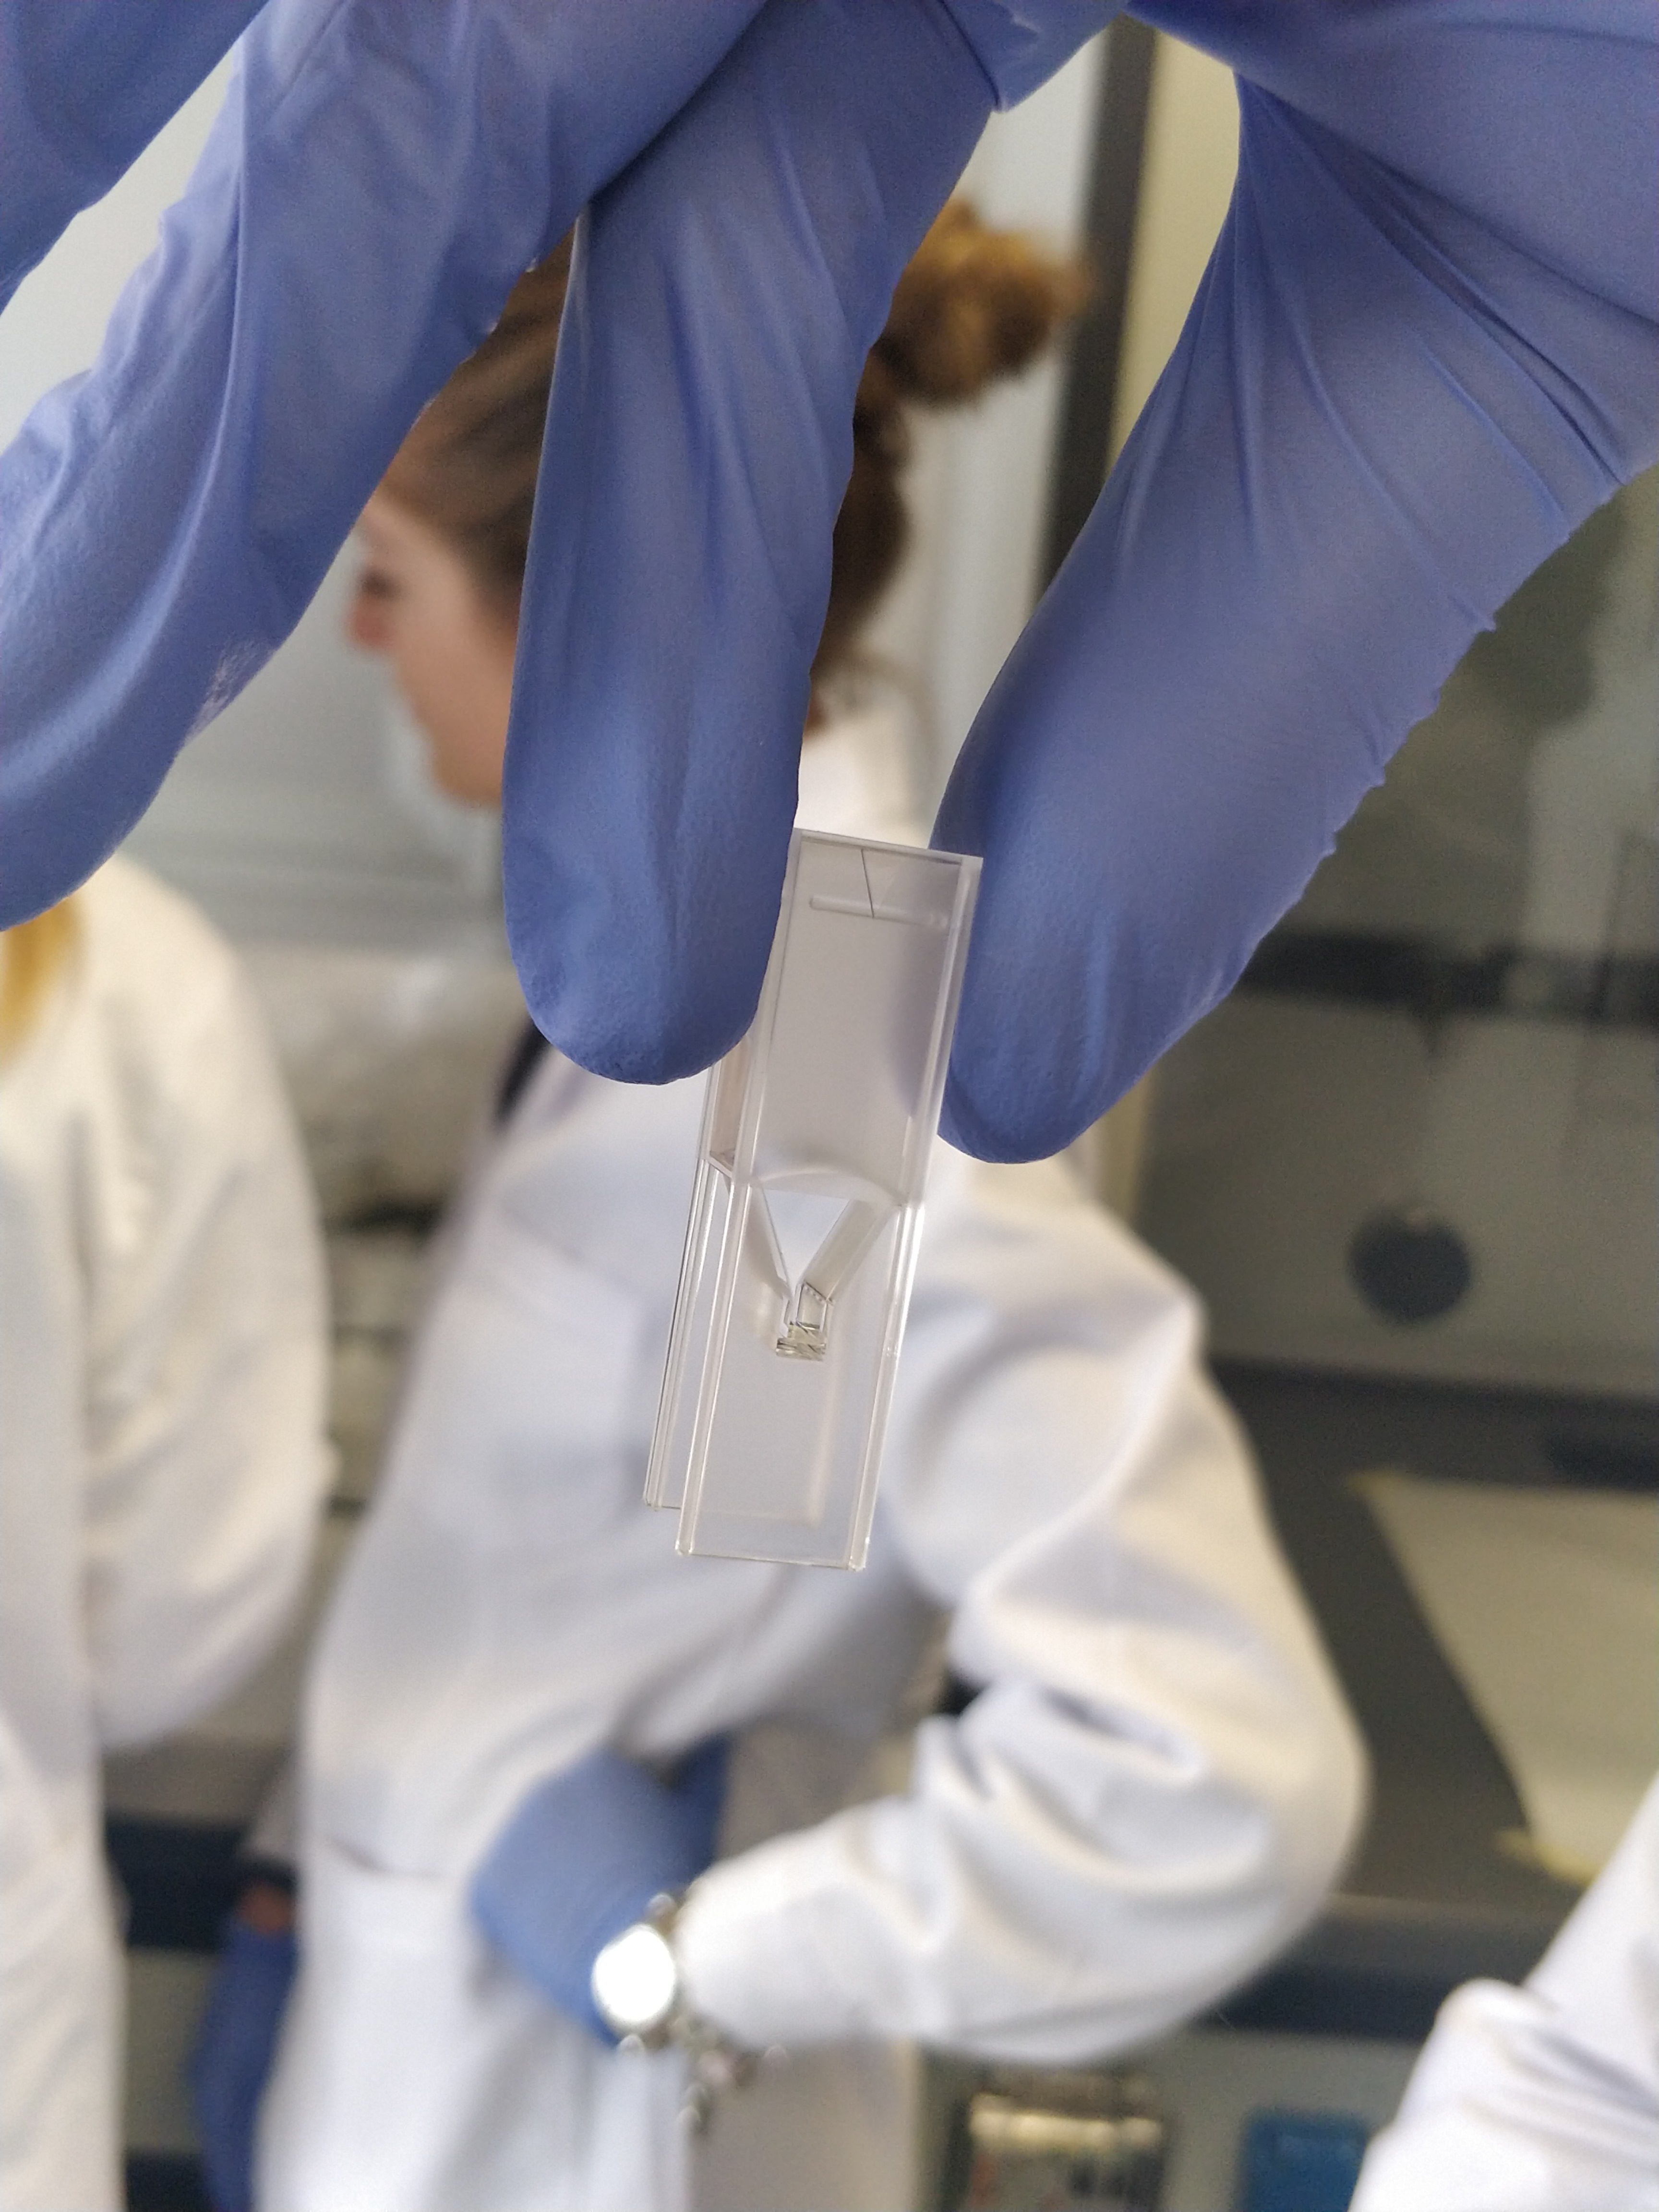
\includegraphics[width=0.3\textwidth]{./immagini/cuvetta.jpg}
\caption{Cuvetta inserita all'interno dello spettrofotometro}
\label{cuvetta}

\end{figure}

\textbf{Spettrofotometro NanoDrop}
\vspace{0.5cm}
Misurazione della concentrazione di pUC18 (riferimento alla prima esperienza)
\begin{enumerate}
\item Depositare una goccia (\SI{2}{\micro\liter}) di acqua sul tip del Nanodrop.
\item Abbassare il braccio delicatamente e registrare il bianco.
\item Sollevare il braccio ed asciugare il tip con della carta assorbente.
\item Depositare una goccia di campione sul tip del nanodrop.
\item Abbassare delicatamente il braccio e registrare il risultato dello spettro.
\item Calcolare la quantità di RNA e la sua purezza, poi congelare l’RNA non diluito e il plasmide pUC18.
\item Alla fine congelare l'RNA non diluito ed il plasmide pUC18.
\end{enumerate}


\section{Risultati e conclusioni}
\begin{table}[H]
\begin{center}

\caption{Risultati Spettrofotometro a Cuvetta.}
\vspace{0,3cm}
\begin{tabular}{lrrrrr}
   & \multicolumn{1}{c}{Risultati allo spettrofotometro} \\
   Esame & \multicolumn{1}{c}{I} \\ \hline
    & & & & & \\

  A280 & $0,016$  \\
 A260 & $0,01$   \\ \\ \hline
       & & & & & \\
  & & & & &  \\ \multicolumn{6}{l}{\small Fonte: Dati dal laboraorio}
\end{tabular}

\end{center}
\end{table}

Per trovare la purezza dell'RNA \`e necessario tener conto delle diluizioni fatte, quindi:\\
$0,016 x 20 = 0,32$ e $0,01 x 20 = 0,002$ in fine si fa il rapporto: $0,32/0,2 = 1,6$

\begin{table}[H]
\begin{center}

\caption{Risultati di quantificazione al NanoDrop.}
\vspace{0,3cm}
\begin{tabular}{lrrrrr}
   & \multicolumn{1}{c}{Risultati al Nanodrop} \\
   Esame & \multicolumn{1}{c}{I} \\ \hline
    & & & & & \\

  A260 /A280 & $1,96$  \\
 A260/A230 & $2,34$   \\
  ng/uL & $127,5$   \\ \\ \hline
       & & & & & \\
  & & & & &  \\ \multicolumn{6}{l}{\small Fonte: Dati dal laboratorio}
\end{tabular}

\end{center}
\end{table}

Dai dati risulta che il nostro campione è composto da pochissimo RNA,
ma l'RNA estratto ha un grado di purezza molto elevato.
